\section{Strojno ucenje}

\subsection{Evalviranje hipotez}
Pomembni kriteriji:
\begin{itemize}
    \item \textbf{konsistentnost} hipotez z primeri (ucnimi)
    \item \textbf{splosnost} (tocnost za nevidene primere)
    \item \textbf{razumljivost} hipotez
\end{itemize}
\green{TP}=true positive, \green{TN}-true negative, \green{FP}-false positive (\blue{napaka 1. tipa}), \green{FN}-false negative (\blue{napaka 2. tipa}) \\
$\text{\green{Klasifikacijska tocnost}}=\frac{TP+TN}{TP+TN+FP+FN}=\frac{TP+TN}{N}$\\
$\text{\green{Obcutljivost/senzitivnost}}=TPR=\frac{TP}{TP+FN}$

\subsubsection{Binarizacija atributov}
Aleternativa za resevanje problematike z vecvrednostnimi atributi:\\
\blue{Strategije} (za primer B = \{Y, G, R, B\}):
\begin{itemize}[leftmargin=*,topsep=0pt,noitemsep]
    \item $\left[\{Y \}, \{R, G, B \} \right]$ (one-vs-all)
    \item $\left[\{Y, R\}, \{G, B\}\right]$ 
    \item vpeljava bianrnih atributov za vsako barvo
\end{itemize}
Primer B = \{Y, G, R\}, konstruiramo 3 nove binarne atribute:\\
$ \begin{matrix} barva \\ Y \\ G \\ R \end{matrix} \rightarrow \begin{tabular}{c|c|c} Y & G & R \\ \hline 1 & 0 & 0 \\ 0 & 1 & 0 \\ 0 & 0 & 1\end{tabular}$
\textbf{Prednost}: manjse vejanje drevesa.

\subsection{Gradnja odlocitvenih dreves}
Drevo gradimo tako da v vsakem koraku izberemo atribut, ki
najvec zmanjsa entropijo (ima najvecji informacijski prispevek).\\
\textbf{Rezidualna entropija} (najbolsi atribut -> najnizja)\\
$\green{H_{\text{rez}}(A)}=-\sum\limits_{a_i\in A}p(A=a_i)\sum\limits_{c_i\in C} p(C=c_i|A=a_i)\log_2p(C=c_i|A=a_i)$\\
\textbf{Informacijski prispevek} (najboljsi atribut maksimizira)\\
$\text{\green{Gain(A)}}=H(\text{Class})-H_{rez}(A)$\\
\textbf{Razmerje inofrmacijskega prispevka atributa A}:\\ 
$\text{\green{IGR(A)}}=\frac{\text{Gain(A)}}{\text{H(A)}}$\\
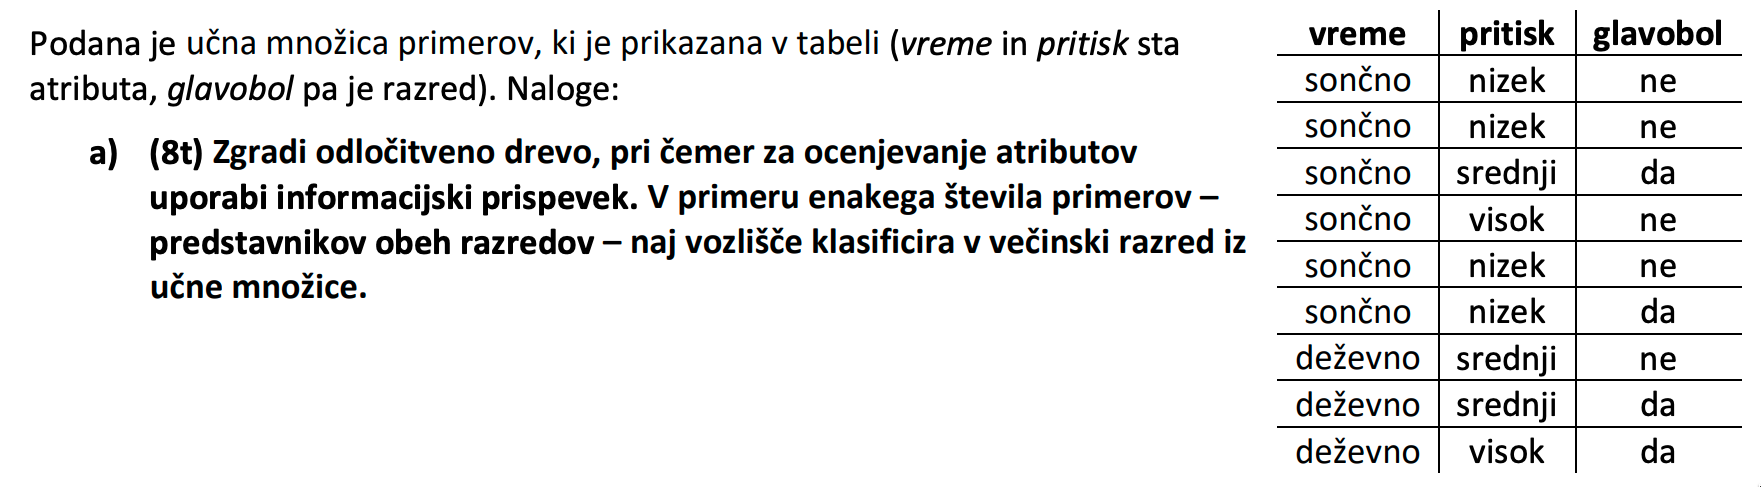
\includegraphics[width=\columnwidth]{./images/decision_tree.png}\\
$H(G)=-\frac{5}{9}\log_2\frac{5}{9}-\frac{4}{9}\log_2\frac{4}{9}=-0.991$\\
$H_{rez}(V)=\frac{3}{9}\left(H(1/3, 2/3)\right) + \frac{6}{9}\left(H(4/6, 2/6)\right)=-0.918$\\
$H_{rez}(P)=\frac{4}{9}\left(H(1/4, 3/4)\right) + \frac{3}{9}\left(H(2/3, 1/3)\right) + \frac{2}{9}\left(H(1/2, 1/2)\right)=0.89$\\
$H_{rez}(P)< H_{rez}(V) \rightarrow$ \textbf{P}ritisk je najboljsi atribut z njim naprej delimo...\\

\subsubsection{TDIDT (Top down induction decision tree) algoritem}
Pozresen algoritem, ki \textbf{lokalno} izbira najbolsi atribut.\\
- kratkoviden algoritem\\
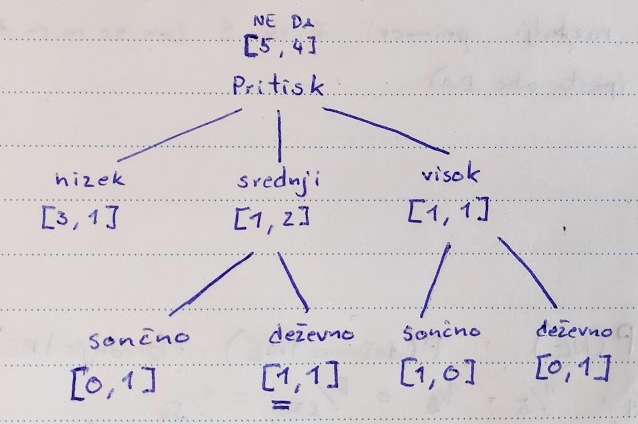
\includegraphics[width=\columnwidth]{images/decision_tree2.png}\\
\textbf{Nizek pritisk} nismo delili naprej, saj nimamo nobenega primera
ki bi imel nizek pritisk in dezevno vreme (samo soncno). Ce bi delili bi
dobili razreda soncno: [3, 1] in dezevno: [0, 0] kar nebi imelo smisla.

\subsection{Ucenje iz sumnih podatkov (rezanje)}
Ucna mnozico razbijemo na: 70\% za gradnjo, 30\% za rezanje. 
\green{Z rezanjem} odstranimo poddrevesa, ki niso kriticna 
in so redundantna tako \textbf{zmansamo velikost drevesa}.\\

\green{tocnost t}...verjetnost pravilnosti klasifikacije\\
\green{napaka e} $\dots$ $1-t$\\
\green{relativna frekvenca} $p=\frac{n}{N}$\\
\green{m-ocena} $p=\frac{n + p_a * m}{N+m}$\\
$m \dots$ koliko zaupam apriorni verjetnosti\\
$p_a$ apriorna verjetnost (pove domenski ekspert) (v nasem primeru relativna frekvenca)\\
\green{Laplacova ocena verjetnosti} $p=\frac{n+1}{N+k}$\\
k...stevilo vseh moznih razredov

\subsubsection{MEP (Minimal Error Prunning)}
\green{e}=staticna napaka, \green{E}=vzvratna napaka, $\green{e\leq E} \rightarrow$ rezemo poddrevo\\
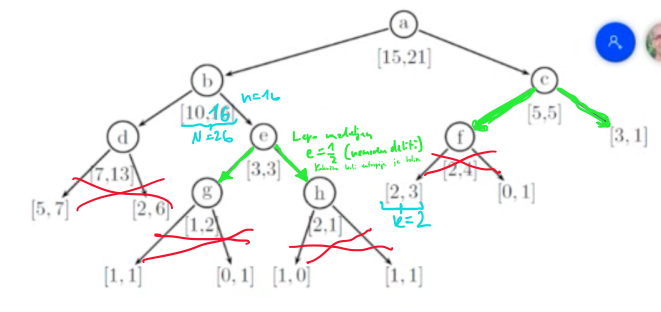
\includegraphics[width=\columnwidth]{./images/mep.png}\\
Primer z (Laplace)\\
$e_L(d)=1-t=1-\frac{13+1}{20+2}=0.363$\\
$E_L(d)=12/20\cdot e_L(d_l) + 8/20\cdot e_L(d_d)= \frac{12}{20} \cdot(1-\frac{7+1}{12+2})+\frac{8}{20}(1-\frac{13+1}{20+2})$\\

\subsubsection{REP (reduced error prunning)} 
G(v)=st. napacnih klasifikacij v poddrevesu - st. napacnih klasifikacij v korenu poddrevesa\\
$G(v)\geq 0 \Rightarrow$ rezemo podrevo\\
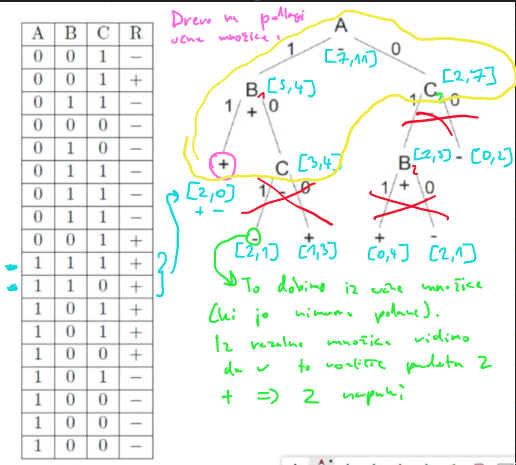
\includegraphics[width=\columnwidth]{./images/rep.png}\\
$e(C)=3$,\;\;\; $e_T=2+3=5$,\;\;\; $G(C)=5-3=2\geq0 \rightarrow \text{rezemo}$

\subsection{Ocenjevanje uspesnosti modelov}
\green{tocnost t} $\dots$ verjetnost pravilnosti klasifikacije\\
\green{Laplacova ocena verjetnosti} $p=\frac{n+1}{N+k}$\\
k...stevilo vseh moznih razredov\\
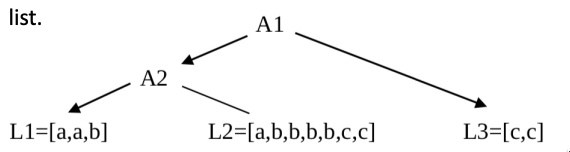
\includegraphics[width=\columnwidth]{./images/drevo-laplace.png}\\
$t_{L1}=\frac{2+1}{3+3}=0.5$,
$t_{L2}=\frac{4+1}{7+3}=0.5$,
$t_{L3}=\frac{2+1}{2+3}=0.6$\\
tocnost drevesa: $t_D=3/12\cdot 0.5 + 7/12\cdot 0.5 + 2/12\cdot 0.6=0.5167$\\
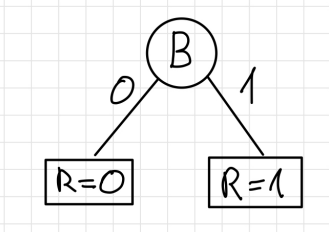
\includegraphics[width=\columnwidth]{./images/klasifikacijska-napaka.png}\\
$e=1-(P(B=0)P(R=0|B=0)+P(B=1)P(R=1|B=1))$

\subsection{Obravnanva mankajocih atributov, navini Bayesov klasifikator}
\subsubsection{Naivni bayes}
Ce poznamo razred, kam klasificiramo ce nepoznamo atributov:\\
\textbf{Klasifikator}: \text{argmax}$_{c\in C} P(c)\prod\limits_{i=1}^n P(x_i|c)$\\
$c\dots \text{razred}$, $x_i\dots \text{atributi}$\\
Verjetnost::\\
$P(C=c|x_1,\dots,x_n)=\frac{P(C=c)P(X_1=x_i|C=c)P(X_2=x_j|C=c)\dots}{P(X_1=x_i)P(X_2=x_j)\dots}$\\


Primer pritisk, vreme, razred glavobol
$$
\begin{array}{|c|c|c|}
    \hline
    X\backslash Y   & \text{ne}      & \text{da}\\
    \hline
    \text{P(G)}           & \text{P(G=ne) = 5/9}    & P\text{(G=da) = 4/9}\\
    \hline
    \text{P(P=srednji)}   & \text{P(P=sre|G=ne)=1/5} & \text{P(P=sre|G=da)=2/4}\\
    \hline
    \text{P(V=dezevno)} & \text{P(V=dez|G=ne)=1/5} & \text{P(V=dez|G=da)=2/4}\\
    \hline
    P(y)\prod\limits_{i=1}^n P(x_i|y) & \text{5/9}\cdot\text{1/5}\cdot\text{1/5} & \text{4/9}\cdot\text{2/4}\cdot\text{2/4}\\
    \hline
\end{array}
$$

\subsubsection{Nomogragmi}
Ciljni razred $C=c_T$\\
$X_{X_i=x_j}=\ln \left( \frac{\frac{P(C=c_T|X_i=x_j)}{P(C=\overline{c_T}|X_i=x_j)}}{\frac{P(C=c_T)}{P(C=\overline{c_T})}} \right) $\\
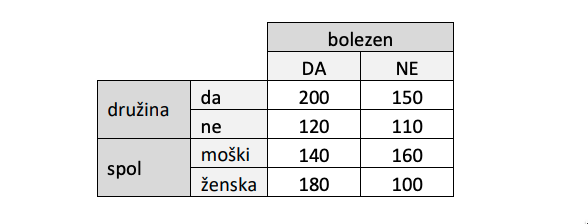
\includegraphics[width=\columnwidth]{images/nomogram.png}\\
Napisi nomogram za verjetnostno razlago modela za klasificiranje v razred \textbf{bolezen=da}\\
$X_{D=da}=\ln \left( \frac{\frac{200}{150}}{\frac{320}{260}}\right) = 0.08$\\
$X_{D=ne}=-0.121$\\
$X_{S=m}=-0.341$\\
$X_{S=z}=0.380$\\
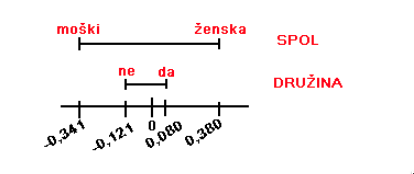
\includegraphics[width=\columnwidth]{images/nomogram2.png}
Da ima oseba \textbf{bolezen} najbolj pripomoreta, da je 
oseba \textbf{zenska} in ima \textbf{druzino}.

\subsection{K-najblizjih sosedov}
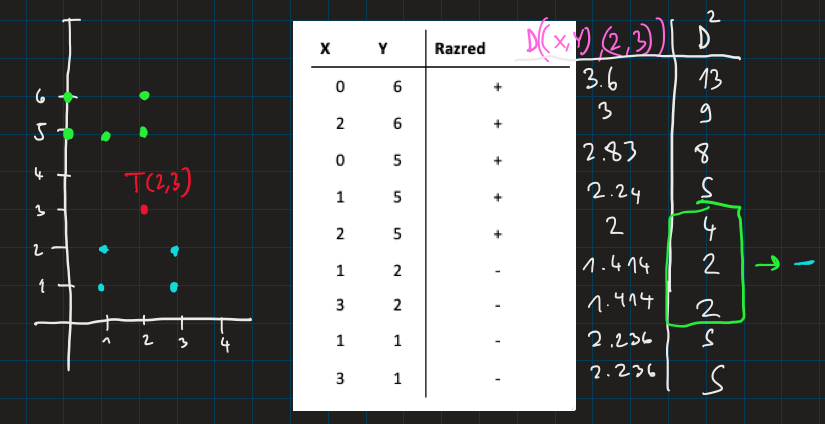
\includegraphics[width=\columnwidth]{./images/knn.png}

\subsection{Regresija}
\textbf{Ucni primeri so podani/oznaceni} kot \textbf{vrednosti vhodov in izhodov}.\\
$(\vec{x}_1,\vec{y}_1),(\vec{x}_2,\vec{y}_2),\dots,(\vec{x}_N,\vec{y}_N)$\\
$\vec{x}_i\dots$ atributi, $\vec{y}_i\dots$ ciljna spremenljivka\\
Locimo dve vrsti problemov:
% Create the list of problems with no margins
\begin{enumerate}[leftmargin=*,noitemsep,topsep=0pt,partopsep=0pt]
    \item \textbf{Klasifikacijski problemi} - $y_j$ \underline{diskretna} 
    \item \textbf{Regresijski problemi} - $y_j$ \underline{zvezna} 
\end{enumerate}

\subsubsection{Lokalno utezena regresija}
$h(\vec{x}_?) = \frac{\sum\limits_{i=1}^k w_i\cdot f(\vec{x}_i)}{\sum\limits_{i=1}^k w_i}, \: w_i(d) ... \text{utez}$\\
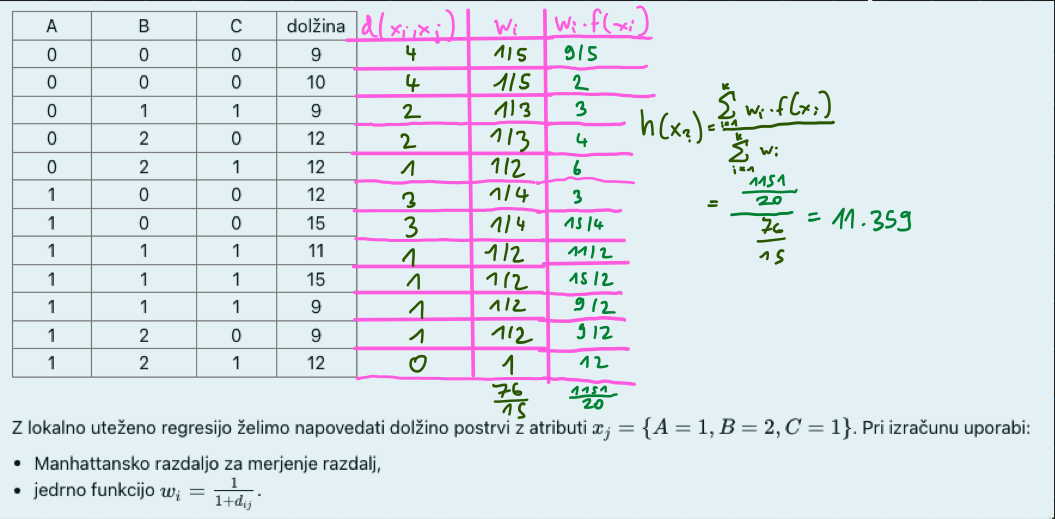
\includegraphics[width=\columnwidth]{./images/lokalno-utezena-regresija.png}

\subsubsection{Regresijska drevesa}
Linearna regresija je poseben primer regresijskega drevesa.\\
V listih regresijskega drevesa vcasih napovemo kar povprecno vrednost.

\subsection{Unsupervised learning}
\textbf{Ucni primeri niso oznaceni} (nimajo ciljne spremenljivke),
\textbf{ucimo se vzorcev v podatkih}, (npr. grucenje)

\subsubsection{Hierarhicno grucenje}
Poveze po podobnosti med primeri, primer zacne kot samostojna gruca, na koncu vsi primeri pripadajo eni gruci\\
\textbf{Dendrogram}: drevo, ki predstavlja grucenje.\\
\textbf{Single-linkage}: povezava med grucami je najkrajsa razdalje med primeroma iz razlicnih gruc.\\
\textbf{Complete-linkage}: najdaljsa razdalja med primeroma iz razlicnih gruc.\\
\textbf{Average-linkage}: povprecna razdalja med primeroma iz razlicnih gruc.\\
Tocke A(3,1),B(1,2),C(3,4),D(5,2),E(1,1), manhattan, complete linkage:\\
\begin{tabular}{c|ccccc}
    & A & B & C & D & E\\
    \hline
    A & 0 & 3 & 3 & 3 & 2\\
    B &   & 0 & 4 & 4 & \underline{1}\\
    C &   &   & 0 & 4 & 5\\
    D &   &   &   & 0 & 5\\
    E &   &   &   &   & 0\\
\end{tabular}
$\rightarrow$
\begin{tabular}{c|cccc}
    & A & BE & C & D\\
    \hline
    A & 0 & \underline{3} & 3 & 3\\
    BE &   & 0 & 5 & 5\\
    C &  &   & 0 & 4\\
    D &   &   &   & 0\\
\end{tabular}
$\rightarrow$
\begin{tabular}{c|ccc}
    & ABE & C & D\\
    \hline
    ABE & 0 & 5 & 5\\
    C &   & 0 & \underline{4}\\
    D &   &   & 0\\
\end{tabular}
$\rightarrow$
\begin{tabular}{c|cc}
    & ABE & CD\\
    \hline
    ABE & 0 & 5\\
    CD &   & 0\\
\end{tabular}


    

\subsubsection{K-means}
1. V prostor dodamo k centroidov, ki predstavljajo gruce.\\
2. Izracunamo ketri centroid je najblizji vsakemu primeru.\\
3. Izracunamo nove centre gruc = $\frac{1}{|G|}\sum\limits_{i\in G} x_i$\\
4. Ponovimo korake 2 in 3 dokler se centri ne premaknejo.\\
V mnozici tock A(3,1),B(1,2),C(3,4),D(5,2),E(1), manhattanska razdalja, zacetni vrednosti centroidov C1(4,4) in C2(5,4).\\
\begin{tabular}{c|c|c|c}
    Tocka & d(X,C1) & d(X,C2) & Gruca\\
    \hline
    A & 4 & 5 & C1\\ 
    B & 5 & 6 & C1\\
    C & 1 & 2 & C1\\
    D & 3 & 2 & C2\\
    E & 6 & 7 & C1\\
    \hline
\end{tabular}\\
V naslednji iteraciji sta koordinati centroidov:\\
$C1=(\frac{3+1+3+1}{4},\frac{1+2+4+1}{4})=(2,2)$ \; in \; $C2=D=(5,2)$ ...

\subsection{Spodbujevalno ucenje - reinforcement learning}
Inteligentni agent se uci iz zaporedja \textbf{nagrad} in \textbf{kazni}

\subsection{Ocenjevanje ucenja}
\textbf{k-fold}, celo ucno mnozico razbij na k disjunktnih podmnozic za vsako od k podmnozic uporabi mnozico kot testno mnozico, preostalih k-1 mnozic kot ucno mnozico.